\newpage
\null
\begin{center}
    \Huge{\textbf{\underline{Chapter 1.1: Uninformed}}}
\end{center}

\setcounter{section}{0}

\vspace{0.35cm}
\section{Searching Algorithms}

\subsection{Simple Search 1}

\begin{algorithm}[ht]
\caption{SS1}
\begin{algorithmic}
\State Open \(\gets\) \{S\};
\vspace{0.1cm}
\While{ Open \(\neq\) nil}
\State N \(\gets\) Remove node from Open;

\vspace{0.07cm}
\If{(GoalTest(N))}
\State return N;
\Else
\State Open \(\gets\) Open \(\bigcup\) MoveGen(N);
\EndIf

\vspace{0.07cm}
\EndWhile

\vspace{0.1cm}
\State return nil;
\end{algorithmic}
\end{algorithm}

\vspace{0.35cm}
\begin{prettyBox}{Issues With SS1}{red}
It can infinitly loop because we aren't keeping track
of node we already seen to fix that we will use another list
to mark seen nodes
\end{prettyBox}

\vspace{0.75cm}
\subsection{Simple Search 2}

\begin{algorithm}[ht]
\caption{SS2}
\begin{algorithmic}
\State Open \(\gets\) \{S\};
\State Closed \(\gets\) \{\}; \Comment{Seen Node List}
\vspace{0.1cm}
\While{ Open \(\neq\) nil}
\State N \(\gets\) Remove node from Open;

\vspace{0.07cm}
\If{(GoalTest(N))}
\State return N;
\Else

\State Closed \(\gets\) Closed \(\bigcup\) \{N\};
\State Open \(\gets\) Open \(\bigcup\) ( MoveGen(N) \textbackslash\hspace{0.1cm}(Open \(\bigcup\) Closed)); \Comment{Append With No Duplicates}
\EndIf

\vspace{0.07cm}
\EndWhile

\vspace{0.1cm}
\State return nil;
\end{algorithmic}
\end{algorithm}


\begin{prettyBox}{Issues with SS2}{red}
Issue is the current algo only return the goal state and not the path,
this would be enough if we are in the context of configuration problem
but in case of planning problem we must have the path to fix that we will use
current parent node pair representation
\end{prettyBox}

\vspace{0.35cm}
\begin{center}
    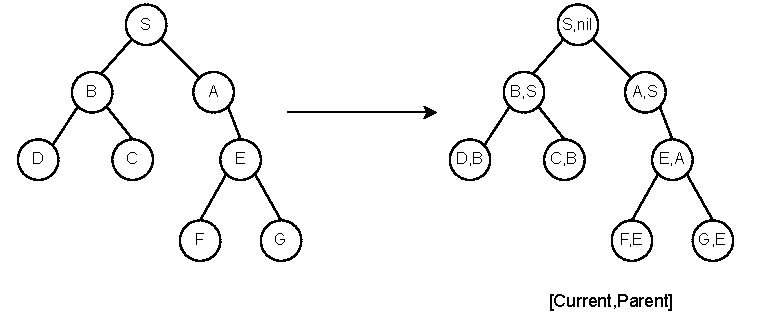
\includegraphics[height=0.3\textheight]{Chapters/Diagram/parent.drawio.pdf}
\end{center}



\vspace{0.5cm}
\subsection{Simple Search 3}

\begin{algorithm}[ht]
\caption{SS3}
\begin{algorithmic}
\State Open \(\gets\) \{\{S,nil\}\};
\State Closed \(\gets\) \{\};
\vspace{0.1cm}
\While{ Open \(\neq\) nil}
\State N \(\gets\) Remove node from Open;

\vspace{0.07cm}
\If{(GoalTest(N.current))}
\State return reconstructPath(N, Closed);
\Else

\State Closed \(\gets\) Closed \(\bigcup\) \{N\};
\State Open \(\gets\) Open \(\bigcup\) ( MoveGen(N) \textbackslash\hspace{0.1cm}(Open \(\bigcup\) Closed));
\EndIf

\vspace{0.07cm}
\EndWhile

\vspace{0.1cm}
\State return nil;
\end{algorithmic}
\end{algorithm}

\newpage
\null
\begin{algorithm}[ht]
\caption{reconstructPath}
\begin{algorithmic}
\Function{reconstructPath}{(I/N:(current,parent),Closed : List{(current,parent)}): List}
\State path \(\gets\) \{N.Current\};
\State N \(\gets\) find node in Closed where N.parent = Closed.current 
\vspace{0.1cm}
\While{ N.parent \(\neq\) nil}
\State path \(\gets\) path \(\bigcup\) \{N.Current\};
\State N \(\gets\) find node in Closed where N.parent = Closed.current 
\EndWhile
\vspace{0.1cm}
\State return reverse(Path);
\EndFunction
\end{algorithmic}
\end{algorithm}

\vspace{0.35cm}

\begin{prettyBox}{How To Choose N}{red}
We have two choices for selecting \( N \): either the head or the tail. The behavior of each choice differs as follows:
\begin{itemize}
    \item \textbf{Head:} If we choose the head, it is treated as a queue. In this case, we \textit{reappend} the state to the end of the structure, effectively following a breadth-first search approach.
    \item \textbf{Tail:} If we choose the tail, it is treated as a stack. We simply \textit{append} the state to the end of the structure, following a depth-first search approach.
\end{itemize}
\end{prettyBox}

\vspace{0.75cm}
\subsection{BFS}
\begin{algorithm}[ht]
\caption{BFS}
\begin{algorithmic}
\State Open \(\gets\) \{\{S,nil\}\};
\State Closed \(\gets\) \{\};
\vspace{0.1cm}
\While{ Open \(\neq\) nil}
\State N \(\gets\) Head(Open);

\vspace{0.07cm}
\If{(GoalTest(N.current))}
\State return reconstructPath(N, Closed);
\Else
\State Closed \(\gets\) Closed \(\bigcup\) \{N\};
\For{ each new in MoveGen(N.current) }
\If{new \(\notin\) Open \(\bigcup\) Closed}

\State Open \(\gets\) Preappend ({new,N});
\EndIf
\EndFor
\EndIf

\vspace{0.07cm}
\EndWhile

\vspace{0.1cm}
\State return nil;
\end{algorithmic}
\end{algorithm}


\newpage


\subsection{DFS}
\begin{algorithm}[ht]
\caption{DFS}
\begin{algorithmic}
\State Open \(\gets\) \{\{S,nil\}\};
\State Closed \(\gets\) \{\};
\vspace{0.1cm}
\While{ Open \(\neq\) nil}
\State N \(\gets\) Tail(Open);

\vspace{0.07cm}
\If{(GoalTest(N.current))}
\State return reconstructPath(N, Closed);
\Else

\State Closed \(\gets\) Closed \(\bigcup\) \{N\};
\For{ each new in MoveGen(N.current) }
\If{new \(\notin\) Open \(\bigcup\) Closed}
\State Open \(\gets\) Append ({new,N});
\EndIf
\EndFor
\EndIf

\vspace{0.07cm}
\EndWhile

\vspace{0.1cm}
\State return nil;
\end{algorithmic}
\end{algorithm}


\vspace{0.35cm}

\subsubsection{Bounded DFS}

\begin{algorithm}[ht]
\caption{Bounded DFS}
\begin{algorithmic}
\State Open \(\gets\) \{\{S,nil, 0\}\};  \Comment{Add depth information}
\State Closed \(\gets\) \{\};
\State Bound \(\gets\) \text{max depth};
\vspace{0.1cm}
\While{ Open \(\neq\) nil}
    \State N \(\gets\) Tail(Open);
    \State Depth \(\gets\) N.depth;  \Comment{Get current depth}

    \If{(GoalTest(N.current))}
        \State return reconstructPath(N, Closed);
    \ElsIf{Depth \(\leq\) Bound}  \Comment{Check if depth is within the bound} 
    \State Closed \(\gets\) Closed \(\bigcup\) \{N\};
    \For{ each new in MoveGen(N.current) }
            \If{new \(\notin\) Open \(\bigcup\) Closed}
                \State Open \(\gets\) Append ({new, N, Depth+1});
            \EndIf
        \EndFor
    \EndIf
\vspace{0.07cm}
\EndWhile
\vspace{0.1cm}
\State return nil;
\end{algorithmic}
\end{algorithm}

\newpage

\subsubsection{DFID}

\begin{algorithm}[ht]
\caption{DFID}
\begin{algorithmic}
\State db \(\gets\) 0;
\While{BDFS(db) = nil}
\State++db;
\EndWhile
\end{algorithmic}
\end{algorithm}

\vspace{0.35cm}

\begin{table}[ht]
\centering
\begin{tabular}{|c|c|c|c|c|}
\hline
\textbf{Algorithm} & \textbf{Space Complexity} & \textbf{Time Complexity} & \textbf{Completeness} & \textbf{Optimality} \\
\hline
\textbf{BFS} & \( O(b^d) \) & \( O(b^d) \) & Yes & Yes \\
\hline
\textbf{DFS} & \( O(bm) \) & \( O(b^m) \) & No & No \\
\hline
\textbf{Bounded DFS} & \( O(b \cdot d) \) & \( O(b^d) \) & No & No \\
\hline
\textbf{DFID} & \( O(b \cdot d) \) & \( O(b^d) \) & Yes & Yes \\
\hline
\end{tabular}
\end{table}

\begin{prettyBox}{Note}{red}
\begin{itemize}
    \item b :  branch factor, max number of children node has 
    \item d : deepth ,max edges between nodes
    \item Completness : Find The Solution if it exist
    \item Optimal : if it result in shortest path
\end{itemize}
\end{prettyBox}
